\documentclass[tikz,border=0pt]{standalone}
\usepackage[american]{circuitikz}
\usetikzlibrary{arrows.meta,calc,positioning,decorations.pathmorphing,patterns}
\definecolor{zyloTeal}{HTML}{174A5B}
\definecolor{zyloTealTwo}{HTML}{246B7A}
\definecolor{zyloInk}{HTML}{1F2933}
\definecolor{zyloSoft}{HTML}{EAF4F4}
\definecolor{zyloPaper}{HTML}{F8FAFB}
\definecolor{zyloLine}{HTML}{44606B}
\definecolor{zyloOrange}{HTML}{D97706}
\begin{document}
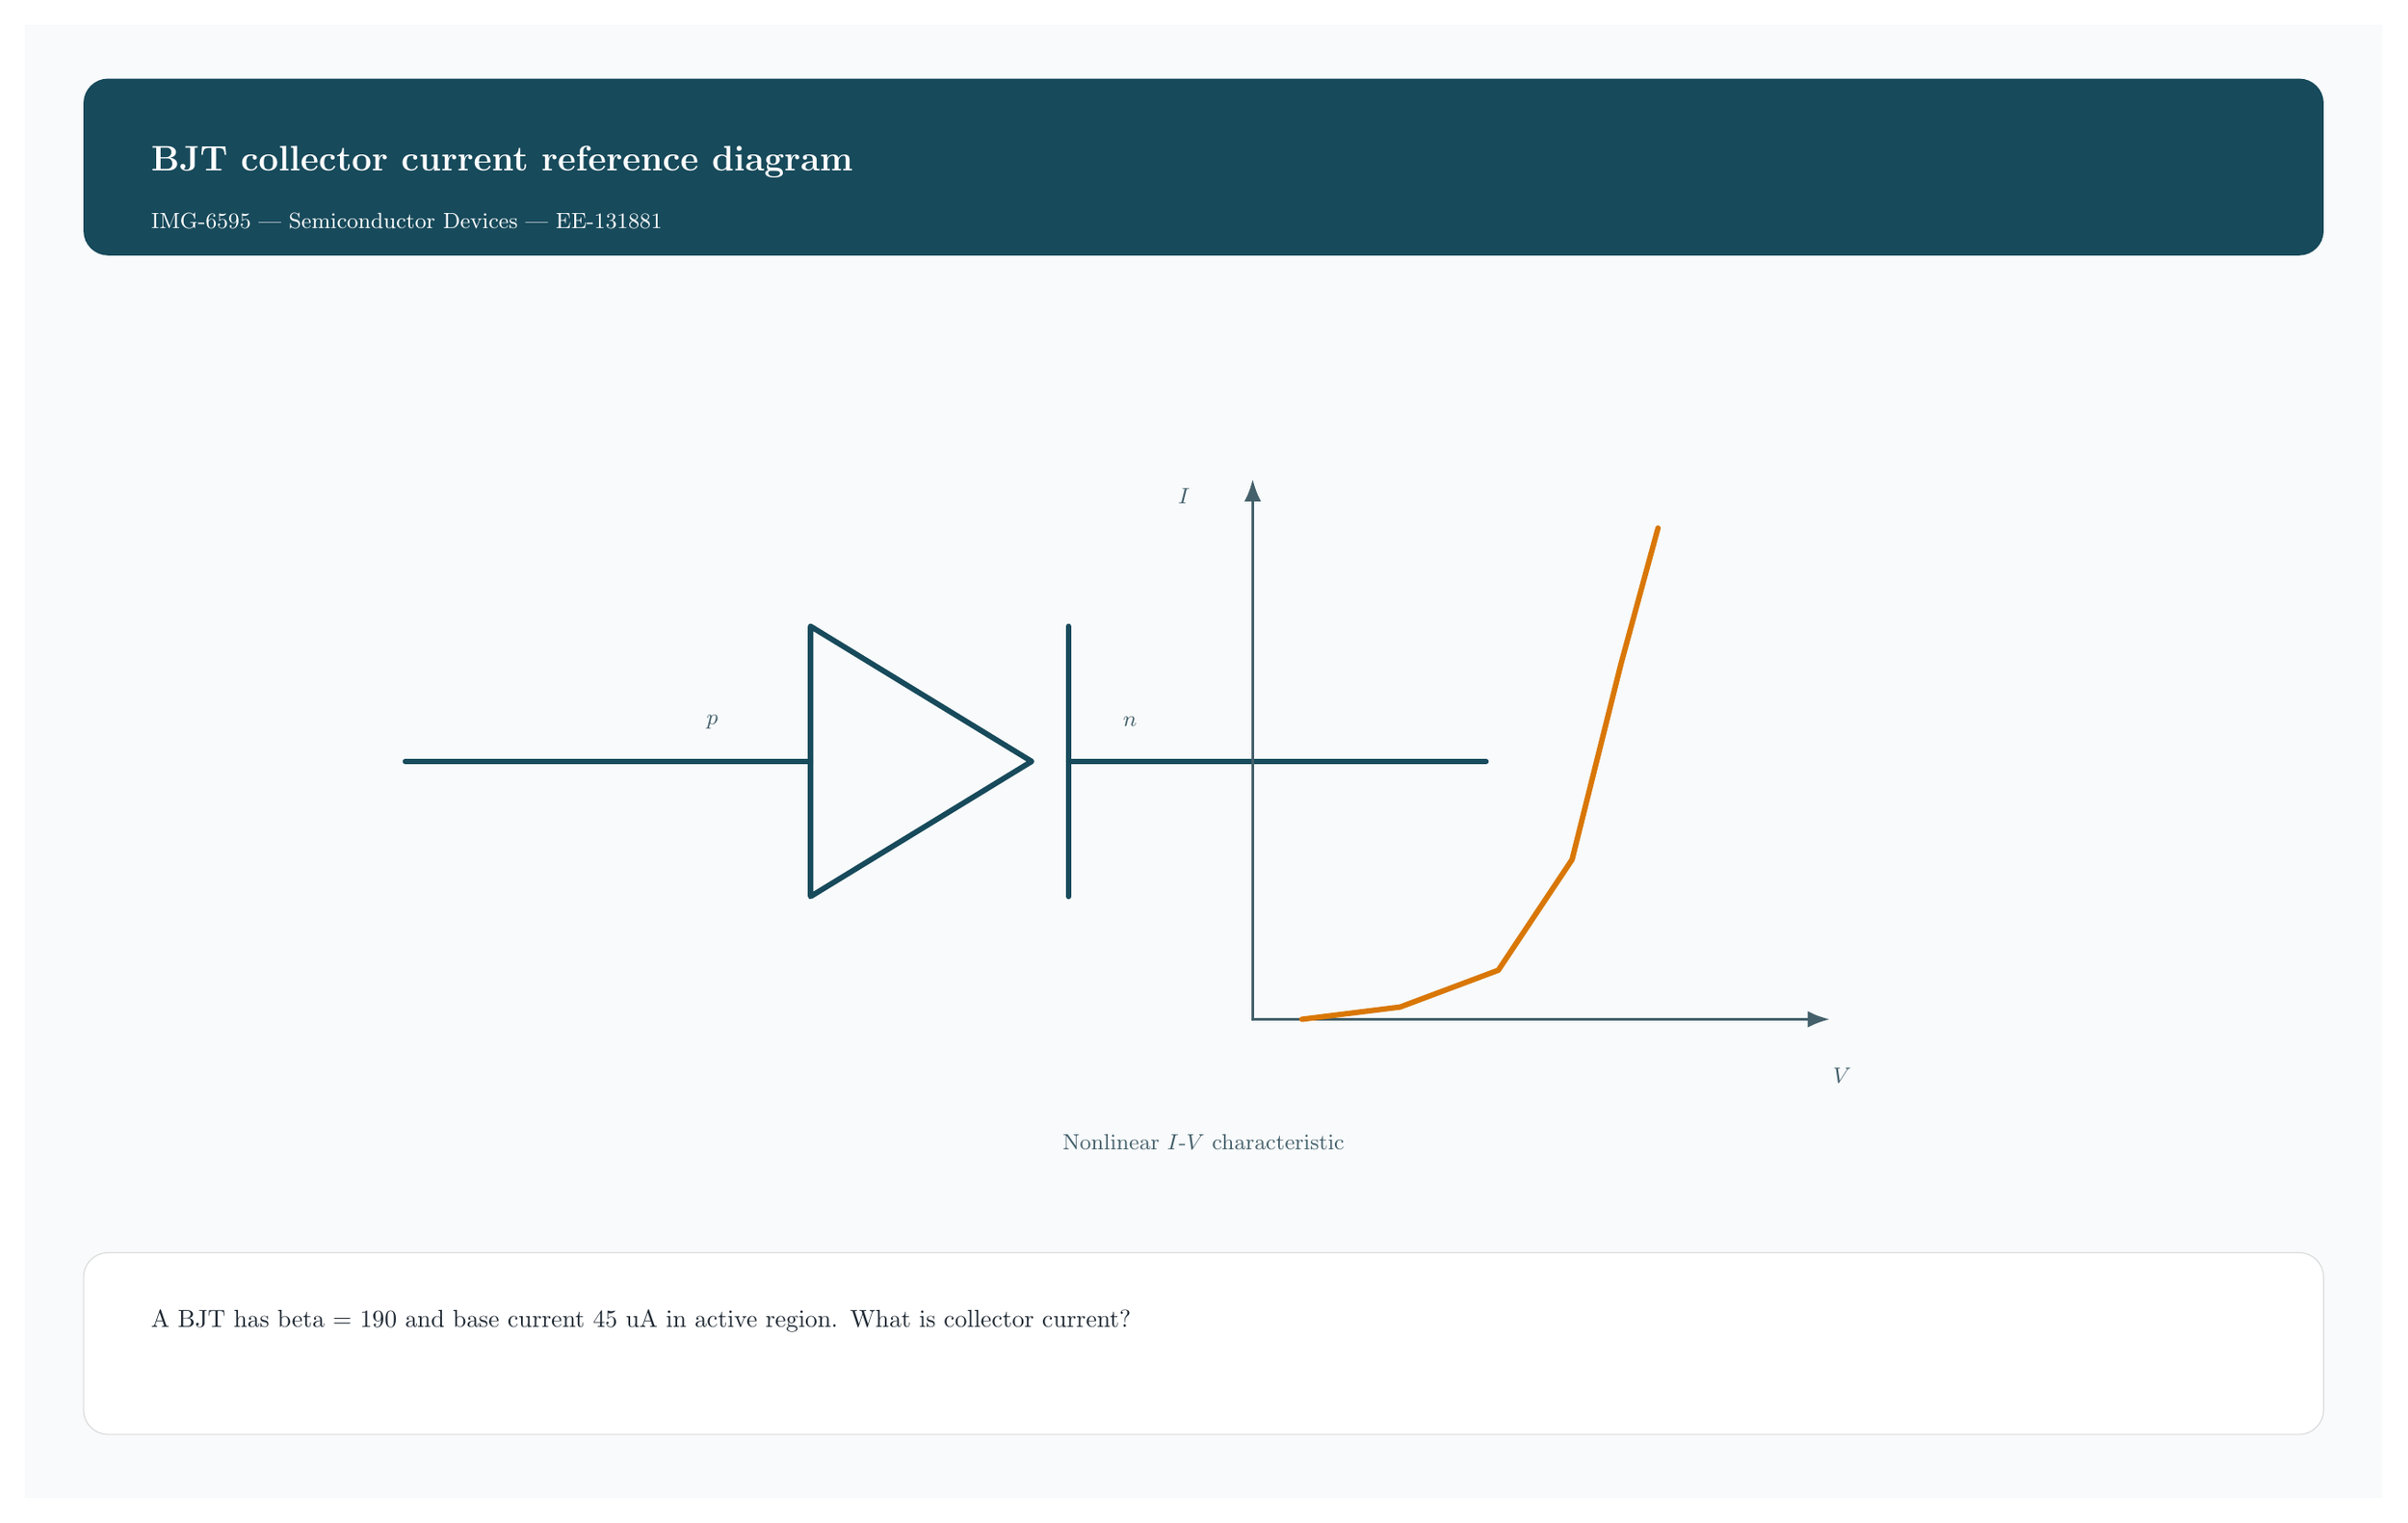
\begin{tikzpicture}[x=1pt,y=-1pt,>=Latex,line cap=round,line join=round]
\path[fill=zyloPaper] (0,0) rectangle (960,600);
\path[fill=zyloTeal,rounded corners=10pt] (24,22) rectangle (936,94);
\node[anchor=west,text=white,font=\bfseries\Large] at (48,56) {BJT collector current reference diagram};
\node[anchor=west,text=white!82,font=\small] at (48,80) {IMG-6595 | Semiconductor Devices | EE-131881};
\tikzset{wire/.style={draw=zyloTeal,line width=2.2pt},thinwire/.style={draw=zyloLine,line width=1.35pt},accent/.style={draw=zyloOrange,line width=2.2pt},box/.style={draw=zyloTealTwo,fill=zyloSoft,line width=1.5pt,rounded corners=8pt}}
\draw[wire] (155,300) -- (320,300);
\draw[wire] (320,245) -- (320,355) -- (410,300) -- (320,245);
\draw[wire] (425,245) -- (425,355);
\draw[wire] (425,300) -- (595,300);
\node[font=\small,text=zyloLine] at (280,284) {$p$}; \node[font=\small,text=zyloLine] at (450,284) {$n$};
\draw[thinwire,->] (500,405) -- (735,405); \draw[thinwire,->] (500,405) -- (500,185);
\draw[accent] (520,405) -- (560,400) -- (600,385) -- (630,340) -- (650,260) -- (665,205);
\node[font=\small,text=zyloLine] at (740,428) {$V$}; \node[font=\small,text=zyloLine] at (472,192) {$I$};
\node[font=\small,text=zyloLine] at (480,455) {Nonlinear $I$-$V$ characteristic};
\path[draw=black!15,fill=white,rounded corners=10pt] (24,500) rectangle (936,574);
\node[anchor=west,text width=860pt,align=left,text=zyloInk,font=\normalsize] at (48,528) {A BJT has beta = 190 and base current 45 uA in active region. What is collector current?};
\end{tikzpicture}
\end{document}
